\documentclass[a4paper, 11pt]{article}

% Fonts 
\usepackage{opensans}
\usepackage{amsfonts}
\usepackage{montserrat}
\usepackage{amsmath}

\usepackage[mathrm=sym]{unicode-math}

\setmainfont{opensans}
\setmathfont{Fira Math}

\newfontfamily{\montserrateb}{Montserrat SemiBold}
\newfontfamily{\montserratb}{Montserrat Bold}
\newfontfamily{\montserrat}{Montserrat Regular}
\newfontfamily{\montserratl}{Montserrat Light}
\DeclareMathAlphabet{\mathcal}{OMS}{cmbrs}{m}{n}

% \autoref
\usepackage{hyperref}

% Use for [H] option for figures to force in text placement
\usepackage{float}

% Captioning figures
\usepackage{caption}

% Subfigures
\usepackage{subcaption}

% For extending contents beyond margins
\usepackage{scrextend}

% For tables \midrule ect
\usepackage{booktabs}

% Colours
\usepackage[table,xcdraw]{xcolor}
\definecolor{accentcolor}{HTML}{6332a8}

% Change label in enumerate 
\usepackage{enumitem}

% Section settings
\usepackage{titlesec}
\titleformat{\section}
{\LARGE\montserrateb}
{\thesection.}{0.5em}{}

\titleformat{\subsection}
{\large\montserratb}
{\thesubsection.}{0.5em}{}

% Adjust document dimensions
\ExecuteOptions{a4paper}
\addtolength{\oddsidemargin}{-3cm} 
\addtolength{\evensidemargin}{-3cm}
\addtolength{\topmargin}{-3cm} 
\addtolength{\textwidth}{6cm}
\addtolength{\textheight}{4.5cm}
\addtolength{\textheight}{1.5cm}
\addtolength{\headsep}{-0.5cm}
% \addtolength{\footskip}{-1cm}
\parindent0pt
\parskip=4pt



\usepackage{tikz}
\usetikzlibrary{arrows.meta,arrows}
\newcommand*{\TickSize}{0}%

\newcommand*{\AxisMin}{0}%
\newcommand*{\AxisMax}{0}%




\newcommand*{\DrawVerticalPhaseLine}[7][]{%
    \gdef\AxisMin{#5}%
    \gdef\AxisMax{#6}%
    \gdef\TickSize{#7}


    \edef\MyList{#2}% Allows for #1 to be both a macro or not
    \foreach \X in \MyList {
      \draw  (-\TickSize,\X) -- (\TickSize,\X) node [right] {$#1\;=\X$};
      % \node [circle, fill:radius 5pt] at (0,\X) {$y=\X$};
    }

    \edef\MyList{#3}% Allows for #2 to be both a macro or not
    \foreach \X in \MyList {% Up arrows
      \draw [-{Latex[length=2mm, width=2mm]}] (0,\X-0.2) -- (0,\X);
    }

    \edef\MyList{#4}% Allows for #3 to be both a macro or not
    \foreach \X in \MyList {% Down arrows
      \draw [-{Latex[length=2mm, width=2mm]}] (0,\X+0.2) -- (0,\X);
    }

    \draw  (0,\AxisMin) -- (0,\AxisMax) node [above] {#1};
}%

\usepackage{mdframed}

% Creates coloured title box
\newcommand{\thetop}[5]{
    \begin{addmargin}[\oddsidemargin]{\oddsidemargin}
        \colorbox{#5}{\color{white}
          \hbox to \paperwidth{
            \vbox {
              \begin{center}
                {\large\montserratl #1}\\
                \vspace{4pt}
                {\huge\montserratb #2}\\
                {\montserratb #3}\\
                \vspace{-0.5em}
                \rule{20em}{1pt}     
      
                {\large\montserratl 
                    #4
                }
              \end{center}
            }
          }
        }
    \end{addmargin}
}

\newcommand{\NN}{\mathbb{N}}
\newcommand{\ZZ}{\mathbb{Z}}
\newcommand{\RR}{\mathbb{R}}
\newcommand{\CC}{\mathbb{C}}
\newcommand{\dydt}{\frac{dy}{dt}}
\newcommand{\dxdt}{\frac{dx}{dt}}
\def\set#1{\left\{ #1 \right\}}

\begin{document}
\thetop{Robert Christie}{MATHS 260}{S1 2023}{Assignment 2\\Due: 14-05-2023}{accentcolor}


\section*{Q1}
\begin{enumerate}[label=(\alph*)]
  \item We create a plot of the equation for the model, this is shown in \autoref{fig:desmos} for parameter values of $s=0$ and $s=3$. 
  \begin{figure}[H]
    \centering
    \begin{minipage}{0.5\textwidth}
      \includegraphics*[width=\textwidth]{images/graph.eps}
      \caption{Plot of $\frac{dg}{dt}$ (vertical axis) against $g$ (horizontal axis) for $s=0$ and $s=3$ respectively. Units are as provided by the question.}
      \label{fig:desmos}
    \end{minipage}
  \end{figure}
  
  Equilibria occur when $\frac{dg}{dt}=0$, for $s=0$: 
  \begin{alignat*}{2}
    & 0 &=& -g+\frac{10g^2}{16+g^2}+0  \\
    \implies & g &=& g\frac{10g}{16+g^2}  
  \end{alignat*}
  So $g=0$ is one root, otherwise $g\neq0$, so we may divide both sides by $g$: 
  \begin{alignat*}{2}
    & 1 &=& \frac{10g}{16+g^2}  \\
    \implies & 16+ g^2 &=& 10g\\
    \implies & 0 &=& g^2 - 10g + 16
  \end{alignat*}
  Thus: 
  \begin{align*}
    g &=\frac{10\pm\sqrt{(-10)^2-4\cdot 1\cdot16}}2\\
      &= 5\pm \sqrt{\frac{100-64}4}\\
      &= 5\pm \sqrt{9}\\
      &= 5\pm 3
  \end{align*}
  Thus the model has three equilibria when $s=0$ at $g=0$, $g=2$ and $g=8$. We see that as $16+g^2>16$, the fraction $\frac {10g^2}{16+g^2}$ is continuous, as the other parts are also "nice", the whole equation is continuous. Therefore, the sign of $\frac{dg}{dt}$ cannot change sign between equilibria, allowing us to draw a phase line.

  We see that: 
  \begin{align*}
    \text{At $g=-1$}\quad & \frac{dg}{dt}=  1+\frac{10}{16+1}>0\\
    \text{At $g=1$ }\quad & \frac{dg}{dt}= -1+\frac{10}{16+1}<0
    \text{At $g=5$ }\quad & \frac{dg}{dt}= -5+\frac{10\cdot 25}{16+25}>0\\
    \text{At $g=10$}\quad & \frac{dg}{dt}=-10+\frac{10\cdot100}{16+100}<0
  \end{align*}

  From this we can determine the type of equilibria and plot the phase line for the model at $s=0$:

  \begin{figure}[H]
    \centering
    \begin{minipage}[c]{0.2\textwidth}
      \begin{tikzpicture}[thick,scale=0.5]
        \DrawVerticalPhaseLine[$g$]{0,2,8}{-1,5}{1,9}{-2}{10}{6pt}%
    \end{tikzpicture}
    \end{minipage}%
    \begin{minipage}[c]{0.5\textwidth}
      \begin{itemize}
        \item Sink at $g=0$, as $g$ moves towards $0$ from above and below. 
        \item Source at $g=2$, as $g$ moves away from $2$ above and below. 
        \item Sink at $g=8$, as $g$ moves towards $8$ from above and below. 
      \end{itemize}
    \end{minipage}
 \end{figure}


  \item Now for $s=3$: 
  \begin{alignat*}{2}
            &&    0  &= -g+\frac{10g^2}{16+g^2}+3 \\
  \implies  && (g-3) &= \frac{10g^2}{16+g^2}\\ 
  \implies  && 10g^2 &= (g-3)(16+g^2)\\
  \implies  && 10g^{2}&=g^{3}-3g^{2}+16g-3\cdot16\\
  \implies  && 0&=g^{3}-13g^{2}+16g-48
  \end{alignat*}
  From what we see in the graph in \autoref{fig:desmos}, we expect that $g=12$ may be a root of this cubic, indeed by analysing the coefficients we see that: 
  $$g^{3}-13g^{2}+16g-48 = (g-12)(g^2 -g +4)$$
  Thus $g=12$ is indeed a root, however notice that the discriminant of $g^2 -g +4$ is $(-1)^2-4\cdot 1\cdot 4<0$, thus $g^2 -g +4$ has no real roots and $g=12$ is the only root of $\frac{dg}{dt}$ for $s=3$, thus there is a single equilibrium when $s=3$. 

  As the equations is still autonomous and continuous, we can draw a phase line by checking the sign of $\frac{dg}{dt}$ on each side the of equilibria. 

  \begin{align*}
    \text{At $g=10$}  \quad & \frac{dg}{dt}=  -10+\frac{10\cdot100}{16+100^2}+3>0\\
    \text{At $g=16$ } \quad & \frac{dg}{dt}= -16+\frac{10\cdot16^2}{16+16^2}+3<0
  \end{align*}

  Thus, the only equilibrium is at $g=12$ and is a \textbf{sink}, we can draw a phase line for the system: 

  \begin{center}
    \begin{tikzpicture}[thick,scale=1.5]
      \DrawVerticalPhaseLine[$g$]{12}{11}{13}{10}{14}{2pt}%
    \end{tikzpicture}
  \end{center}






  \item Bifurcations occur when the number of type of equilibria change, for our model this occurs when $s$ is such that the local minima visible in the plot touches the $g$-axis and the derivative transitions between having three roots and one. Desmos gives an approximation of this local minima of $-0.418$, rounded to two decimal places \textbf{the bifurcation occurs at}:
  $$s=0.42$$ 
  
  Before analysing the behaviour of the system as $s$ varies, note that as $16+g^2>g^2\geq0$ it follows that $0\leq\frac{g^2}{16+g^2}\leq1$ so:
  $$0\leq \frac{10g^2}{16+g^2}\leq 10$$

\begin{itemize}
  \item   We can assume that the concentration of the product $g$ is initially $0$. Over time the signal $s$ will rise starting from $s=0$, this will shift the equilibria that initially lies at $g=0$ further to the right. This equilibrium is a sink and so $g$ will stay near it as it moves right causing $g$ to gradually increase until $s$ reaches the bifurcation value.
  
  We can observe from the plot that the local minima occurs below $g=1$ and so the concentration $g$ will increase slowly and remain below $1$ throughout this period.  
  
  \item At the point of bifurcation when $s$ is approximately $0.42$ and $\frac{dg}{dt}>0$ both immediately \textit{above} and \textit{below} the local minima while \textit{at} the minima $\frac{dg}{dt}=0$. Thus, we have a node however, $g$ will still be approaching the node from the left and will only tend to it and not exceed it. This situation only occurs instantaneously assuming $s$ varies continuously. 

  \item Once $s$ exceeds the bifurcation value of approximately $0.42$ a sudden change in behaviour occurs. The node disappears as the local minima remains positive meaning no equilibria are present near this point. 
  
  However, as there are a maximum of three possible equilibria (equilibria were found to be given by roots of cubic) and two are missing due to the local minima been positive, there is only one equilibrium. This equilibrium can be observed in the plot for $s=3$. As we know $\frac{10g^2}{16+g^2}+s$ is between $s$ and $10+s$, for $g<s$ it must be that $g$ is increasing, similarly for $g>10+s$, it must be that $g$ is decreasing. As $g$ can only change directions at equilibria in a continuous model, it must be that around this single equilibrium, $g$ increases below and decreases above making the equilibrium a sink. 
  
  From the plot we can deduce that the single remaining equilibrium will have shifted right from its initial location of $g=8$ when $s=0$, thus the new equilibria which $g$ approaches is at a location of $g>8$. 
  
  Thus, once the bifurcation value is exceeded, the concentration $g$ will rapidly increase approaching the remaining sink. This sudden increase in the concentration of product from $g<1$ to $g>8$ will result in a sudden transition to having grey hair.  

  The concentration $g$ of product will approach somewhere above $8$ and below $12$, once $s$ reaches $3$, the product will be approaching a concentration of $g=12$.
\end{itemize} 


\item Using the qualitative behaviours deduced in previous working we can sketch a bifurcation diagram for the model, this is shown in \autoref{fig:bifurcation}.

\begin{figure}[H]
  \centering
  \begin{minipage}{0.4\textwidth}
    \includegraphics*[width=\textwidth]{images/bifurcation.png}
    \caption{A sketched bifurcation diagram for the model, bifurcations and phase lines for $s<0$ are not drawn as $s$ represents a non-negative quantity.}
    \label{fig:bifurcation}
  \end{minipage}
\end{figure}

By analysing the bifurcation diagram we can deduce that after $s$ passes the bifurcation point $g$ will be near the remaining equilibrium. If $s$ were to decrease, as the equilibrium is a sink, $g$ would follow it. If $s$ were to pass below the bifurcation value, $g$ would still remain close to the largest equilibrium as the location of this equilibrium changes smoothly with $s$ and remains a sink. Even in the even that $s$ were to abruptly drop to $0$, as $g$ would now be above the equilibrium at $8$ which is a sink, it would decrease and tend to $8$, however under no series of signals could the concentration $g$ return below $8$. 

We can conclude that the bifurcation has caused the concentration $g$ to move to a different region, which cannot be escaped even if $s$ returns to a lower value. This makes the transition to grey hair irreversible. (Unless the concentration of product $g$ can be affected directly.) 
\end{enumerate}



\section*{Q2}
\begin{enumerate}[label=(\alph*)]
  \item The associated homogenous equation is: 
  $$
    \frac{dy}{dt}=-y
  $$
  We guess that the one-parameter family given by $\phi(t)=ke^{-t}$ for some parameter $k\in\RR$, are solutions to the homogenous equation, testing this: 
  $$\phi'(t)=-ke^{-t}=-\phi(t)$$ 
  Thus $y_h(t)=\phi(t)$ is indeed the one-parameter family of solutions to the homogenous equation. 

  \item 
  \begin{enumerate}[label=(\roman*)]
    \item We have solutions $y_{p_1}(t)$ and $y_{p_2}(t)$ where:
    \begin{align*}
      y_{p_1}'(t)&=-y_{p_1}(t)+2\cos(3t)\\
      y_{p_2}'(t)&=-y_{p_2}(t)+4t
    \end{align*}
    If we define $y_p:=y_{p_1}+y_{p_2}$, then: 
    $$y_p(t):=y_{p_1}(t)+y_{p_2}(t)$$
    Then we can check that $y_p(t)$ satisfies the non-homogenous DE: 
    \begin{align*}
      y_p'(t)&=y_{p_1}'(t)+y_{p_2}'(t)\\
      &=-y_{p_1}(t)+2\cos(3t)-y_{p_2}(t)+4t\\
      &=-(y_{p_1}(t)+y_{p_2}(t))+2\cos(3t)+4t\\
      &=-y_p(t)+2\cos(3t)+4t
    \end{align*}
    Thus $y_p(t)$ is a particular solution that satisfies the non-homogenous DE. By applying the \textbf{extended linearity principle}, the general solution to the homogenous equations added to any particular solution to the non-homogenous equation is the general solution to the non-homogenous equations. Therefore:
    $$y_h(t)+y_p(t)=y_h(t)+y_{p_1}(t)+y_{p_2}(t)$$
    Gives the general solution to the non-homogenous equation, hence Rey is correct. 

    \item We are trying to find a solution $\phi(t)$ to the DE:
    $$\dydt=-y+2\cos(3t)$$
    For this kind of DE we generally expect we may have a solution of the form: 
    $$\phi(t)=a\sin(3t)+b\cos(3t)$$
    For some constant coefficients $a,b\in\RR$. For $\phi(t)$ to be a solution it must satisfy: 
    \begin{align*}
      \phi'(t)&=-\phi(t)+2\cos(3t)\\
       3a\cos(3t)-3b\sin(3t)  &=-a\sin(3t)-b\cos(3t)+2\cos(3t)\\
       -3b\sin(3t)+3a\cos(3t)  &=-a\sin(3t)+(2-b)\cos(3t)\\
    \end{align*}
    Which is satisfied if and only if: 
    \begin{align*}
      \begin{array}{rcl}
        3b&=&a  \\[6pt]
        3a &=&2-b \\
      \end{array}\implies \begin{array}{rcl}
        9b &=&2-b \\[6pt]
        3b&=&a  \\
      \end{array}\implies \begin{array}{rcl}
        b&=&\frac 15 \\[6pt]
        a&=&\frac 35  \\
      \end{array}
    \end{align*}
    Thus $\phi(t)=\frac 35\sin(3t)+\frac15\cos(3t)$ is a solution to this non-homogenous DE as suggested by Kylo.

    \item Next we find a solution $\phi(t)$ to the non-homogenous DE: 
    $$\dydt=-y+4t$$
    If we were to try:
    $$\phi(t)=4t$$ 
    As our solution we would get $4=-4t+4t$, we see that the $4t$'s on the right cancel nicely only leaving us with a constant on the right to which we also need to remove somehow. 
    
    Note that any constant in $\phi(t)$ will disappear when the derivative is taken and thus leave the left side unaffected, so we try:
    $$\phi(t)=4t-4$$ 
    Thus $\phi'(t)=4$ while $-\phi(t)+4t=-4t+4t+4=4$, thus: 
    $$\phi(t)=4t-4$$
    Is a solution to this non-homogenous equation as Luke suggested. 
  \end{enumerate}
  \item Using the results from part (b):
    $$y(t)=y_h(t)+y_{p_1}(t)+y_{p_2}(t)=ke^{-t}+\frac35\sin(3t)+\frac15\cos(3t)+4t-4$$
  Is a general solution to the non-homogenous DE.
  
  To solve the IVP, we find a value $k\in\RR$ such that $y(0)=-4$:
  \begin{alignat*}{4}
    &        & -4&=y(0)\\
    &\implies& -4&=ke^{-0}+\frac35\sin(0)+\frac15\cos(0)+4\cdot0-4\\
    &\implies& -4&=k+\frac15-4\\
    &\implies&  k&=-\frac15
  \end{alignat*}
  Thus:
  $$y(t)=\frac15e^{-t}+\frac35\sin(3t)+\frac15\cos(3t)+4t-4$$
  Is a solution to the IVP.
  \end{enumerate}


\section*{Q3}
\begin{enumerate}[label=(\alph*)]
  \item We can put the system into matrix form: 
  $$
  \frac{d\mathbf{Y}}{dt}
    =\mathbf{A}
    \mathbf{Y}
  $$
  Where: 
  $$\mathbf{Y}=\begin{bmatrix}
    x \\ 
    y
  \end{bmatrix}\qquad\mathbf{A}=\begin{bmatrix}
    2 & 2\\
    1 & 3
  \end{bmatrix}
  $$
  
  We can find the eigenvalues of $\mathbf{A}$ by finding the roots of the characteristic polynomial: 
  \begin{align*}
    0&=P_\mathbf{A}(\lambda)\\
    &=\det(\mathbf{A}-\lambda \mathbf{I})\\
    &=\det\begin{bmatrix}
      2-\lambda & 2\\
      1 & 3-\lambda
    \end{bmatrix}\\
    &=(2-\lambda)(3-\lambda)-2\\
    &=\lambda^2-5\lambda+6-2\\
    &=\lambda^2-5\lambda+4\\
    &=(\lambda-4)(\lambda-1)\\
  \end{align*}
  So we have eigenvalues $\lambda_1=4$ and $\lambda_2=1$. Now we can find eigenvectors.
  \begin{itemize}
    \item First we find a non-zero $v_1\in\ker(\mathbf{A}-\lambda_1 \mathbf{I})$: 
    \begin{align*}
      0 &= (\mathbf{A}-\lambda_1 \mathbf{I})v_1\\
      &=\begin{bmatrix}
            -2 &  2 \\ 
             1 & -1
          \end{bmatrix}v_1
    \end{align*}
    So $v_1$ is a non-zero solution to: 
    \begin{align*}
      &\left[ 
        \begin{array}{cc|c}
          -2 & 2 & 0 \\
          1 & -1 & 0 \\
        \end{array}
       \right]\\
       \sim&\left[ 
        \begin{array}{rr|r}
          \hphantom{-}1 & -1 & 0 \\
          0 & 0 & 0 \\
        \end{array}
       \right]\quad\begin{array}{l}
        R_1\leftarrow -\frac 12 R_1\\
        R_2\leftarrow R_2 + \frac 12 R_1
       \end{array}
    \end{align*}
    Thus for some non-zero $t\in\RR$:
    \[
     v_1=\begin{bmatrix}
       t \\
       t 
     \end{bmatrix}  \quad\text{Choosing $t=1$:}\quad v_1=\begin{bmatrix}
      1\\
      1
     \end{bmatrix}
    \]
  
    \item Now we find a non-zero $v_2\in\ker(\mathbf{A}-\lambda_2 \mathbf{I})$: 
    \begin{align*}
      0 &= (\mathbf{A}-\lambda_2 \mathbf{I})v_2\\
      &=\begin{bmatrix}
             1 & 2 \\ 
             1 & 2 \\ 
          \end{bmatrix}v_1
    \end{align*}
    So $v_1$ is a non-zero solution to: 
    \begin{align*}
      &\left[ 
        \begin{array}{cc|c}
         1 & 2 & 0 \\
         1 & 2 & 0 \\
        \end{array}
       \right]\\
       \sim&\left[ 
        \begin{array}{rr|r}
          1 & 2 & 0 \\
          0 & 0 & 0 \\
        \end{array}
       \right]\quad\begin{array}{l}
        R_2\leftarrow R_2-R_1
       \end{array}
    \end{align*}
    Thus for some non-zero $t\in\RR$:
    \[
     v_2=\begin{bmatrix}
      -2t \\
       t 
     \end{bmatrix}  \quad\text{Choosing $t=-1$:}\quad v_2=\begin{bmatrix}
      2\\
      -1
     \end{bmatrix}
    \]
  \end{itemize}
  As we have $k=2$ distinct real eigenvalues for our $2\times2$ matrix, the general solution is a two-parameter family is given by: 
  \begin{align*}
    \mathbf{Y}(t) &=c_1e^{\lambda_1t}v_1+c_2e^{\lambda_2t}v_2\quad\text{With two parameters $c_1,c_2\in\RR$}\\
    &=c_1e^{4t}
      \begin{bmatrix}
        1\\
        1
      \end{bmatrix}
      +c_2e^t 
      \begin{bmatrix}
        2\\
        -1
      \end{bmatrix}
  \end{align*}
  Thus the general solution to the system is the two parameter family of two equations with $c_1,c_2\in\RR$: 
  \begin{align*}
    x(t) &= c_1e^{4t}+2c_2e^t\\
    y(t) &= c_1e^{4t}-c_2e^t
  \end{align*}
  
  \item As explained in the part (c), our system has a single equilibrium at the origin which is a source. We know that we have two straight line solutions which lie along the scalar multiplies of each eigenvector. All solutions are linear combinations of these solutions which informs us about the qualitative behaviour of the system. 
  \begin{itemize}
    \item We have straight line solutions that move away from the origin along $y=x$ and $y=-\frac12x$ lines. 
    \item As the component in the general family of solutions from the $v_1$ eigenvectors is given by $v_1e^{4t}$ while the component from the $v_2$ eigenvector is given by $e^t$, as time increases the $e^{4t}$ will grow faster than the $e^{t}$ causing the solutions directions approach parallel to the $\lambda_1$ straight line solution. 
    \item This also means that as time decreases and the non straight line solutions move towards to the origin, the faster $e^{4t}$ decays quicker than $e^t$ and so the solution's behaviour converges on that of the $\lambda_2$ straight line solution as $t\to-\infty$ and $\mathbf{Y}\to0$.
  \end{itemize}
  From these observations we create a phase portrait of the system shown in \autoref{fig:phase}.

  \begin{figure}[H]
    \centering
    \begin{minipage}{0.5\textwidth}
    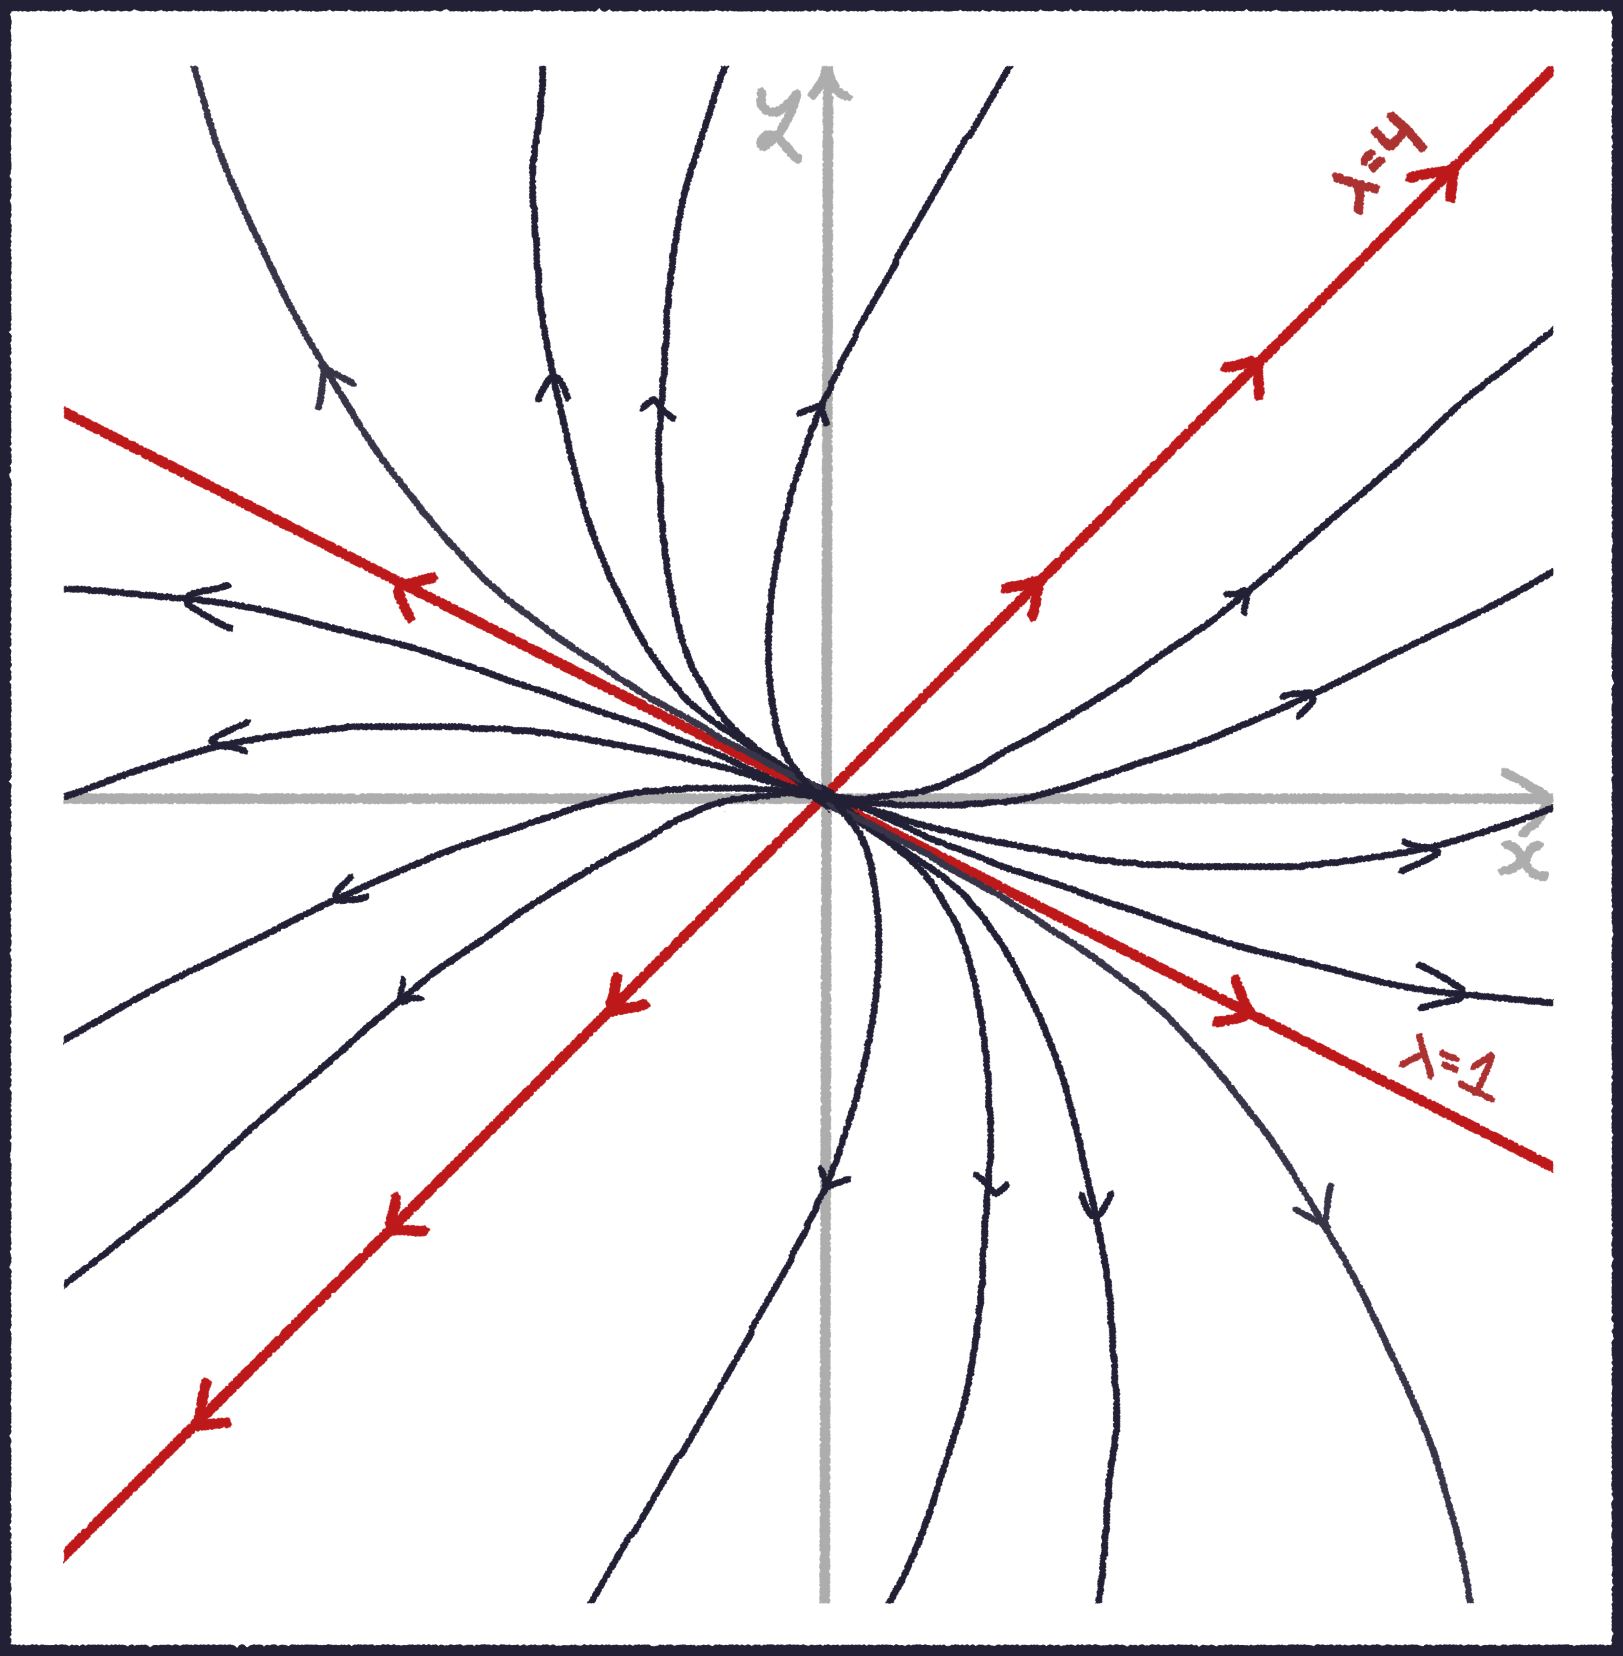
\includegraphics[width=\textwidth]{images/phase.png}
    \caption{Phase portrait of the system in Q3}
    \label{fig:phase}
    \end{minipage}
  \end{figure}

  \item As our system is a constant coefficient linear system of the form: 
  $$\frac{d\mathbf{Y}}{dt}=\mathbf{AY}$$
  Where the eigenvalues of $\mathbf{A}$ are real and distinct, we know that: 
  \begin{itemize}
    \item Our system will have an equilibrium at the origin.
    
    \item At any equilibrium points: 
    $$\frac{d\mathbf{Y}}{dt}=0\implies\dydt=\dxdt=0$$
    Which occurs if and only if: 
    $$2x+2y=0=x+3y\implies x=-y\land x=-3y$$
    Which occurs if and only if $x=y=0$, thus the only equilibrium occurs at the origin.
    
    \item As all eigenvalues of $\mathbf{A}$ are real, distinct, and positive, we know that the system will have a \textbf{source} at the origin and that this is the \textbf{only} equilibrium point in the system. 
  \end{itemize}
\end{enumerate}

\pagebreak
\section*{Q4}
\begin{enumerate}[label=(\alph*)]
  \item \begin{enumerate}[label=(\Roman*)]
    \item \textbf{The carrying capacity of the system is constant.}
    
    The carrying capacity is primarily determined by environmental factors which will have remained relatively constant on Tiritiri Matangi as a result of efforts to protect the ecosystem from invasive species and humans. 
    
    While the carrying capacity is also affect by variations in the climate (different years have varying conditions, drought, excess rain, ect.) and other environmental factors, we assume that these also do not change significantly over the time period we are interested in. 
    
    \item \textbf{The rates of births and deaths per individual both scales linear linearly with population size, giving us a per capita growth rate that scales linearly with the population size. }  
    
    We first assume that per individual, in lower populations that birth rates are higher and death rates lower due to a higher abundance of resources while in larger populations birth rates decrease and death rates increase. Due to an absence of predators on the island this a reasonable assumption as these rates will be primarily determined by the available resources. 

    We also assume that this effect is approximately linear, that the growth rate per individual will decrease linearly as population increases. This assumption is less justified, however, based of previous assumptions we expect this rate to be strictly decreasing as the population increases, this means that a linear approximation will still capture the general behaviour. 
    

    \item \textbf{All individuals reproduce at the same rate.  }
    
    Between individuals of similar age this is a reasonable assumption as even if rates differ the effects will average out given the population is large enough. We know that this will differ over the age of an individual, this could cause significant inaccuracy as similarly sized populations could have significantly different age distribution altering growth rates. We can justify this assumption by assuming that the difference between growth rates is only affected by very old or young individuals which will be relatively few and thus have a minimal impact on accuracy. 

    \item \textbf{The reproduction rate and population are continuous quantities.}
    
    Our model assumes that the system can be modelled by continuous quantities despite the discrete nature of individual birds. This is a good assumption as at the relevant scales the individual impact is insignificant. 
  \end{enumerate}

  \item We choose units to use with the model.
  \begin{itemize}
    \item For population ($P$), we use a unit corresponding to 1000 individuals.
    \item For time ($t$) we use years for our units, we also use years that match the data ($t=2018$ corresponds to the year $2018$). 
  \end{itemize}

  \item Euler's method gives the approximation:
  $$P(t+h)=P(t)+h\cdot\frac{dP}{dt}=P(t)+hkP(t)\left(1- \frac {P(t)}N \right)$$

  Using this approximation with a time step $h=1$, then from the data given we have: 
  \begin{align*}
    P(2019) &= P(2018)+1\cdot k\cdot P(2018)\cdot\left( 1  - \frac{P(2018)}{N} \right)\\
    P(2020) &= P(2019)+1\cdot k\cdot P(2019)\cdot\left( 1  - \frac{P(2019)}{N} \right)
  \end{align*} 

  Filling in the know values in our units:  
  \begin{alignat*}{4}
  && 2.297 &= 1.515+1.515k\left( 1  - \frac{1.515}{N} \right)
  &&\qquad\qquad &
    1.962 &= 2.297+2.297k\left( 1  - \frac{2.297}{N} \right)
  \\
  &\implies&\frac{2.297}{1.515}-1-k &=-k\frac{1.515}{N} 
  &&\qquad\qquad&
    \frac{1.962}{2.297}-1-k &=-k\frac{2.297}{N}
  \\
  &\implies&N &=-k\frac{1.515}{\frac{2.297}{1.515}-1-k} 
  &&\qquad\qquad&
    N &=-k\frac{2.297}{\frac{1.962}{2.297}-1-k}
\end{alignat*} 
Equating both right sides of the equations:
 \begin{alignat*}{2}
  -k\frac{2.297}{\frac{1.962}{2.297}-1-k} &=-k\frac{1.515}{\frac{2.297}{1.515}-1-k}\\
     2.297 k \left( \frac{2.297}{1.515}-1-k \right) 
  &= 1.515 k \left( \frac{1.962}{2.297}-1-k \right) \\
     2.297 \left( \frac{2.297}{1.515}-1-k \right) 
  &= 1.515 \left( \frac{1.962}{2.297}-1-k \right) \\
     2.297 \left( \frac{2.297}{1.515}-1 \right) -2.297k 
  &= 1.515 \left( \frac{1.962}{2.297}-1 \right) -1.515k \\
     1.515k - 2.297k 
  &= 1.515 \left( \frac{1.962}{2.297}-1 \right) -2.297 \left( \frac{2.297}{1.515}-1 \right) \\
  k 
  &= \frac{1.515 \left( \frac{1.962}{2.297}-1 \right) -2.297 \left( \frac{2.297}{1.515}-1 \right)}{1.515 - 2.297} \\
  k &= 1.79871796083\\
    &= 1.799
 \end{alignat*} 


  \item From the previous working we determined that:
  \begin{align*}
    N &=-k\frac{1.515}{\frac{2.297}{1.515}-1-k} =-k\frac{2.297}{\frac{1.962}{2.297}-1-k}\\
      &= 2.12472455604\quad\text{Using determined $k$ to evaluate}\\
      &= 2.125
  \end{align*}
  Note that both expressions give the same value as we set the equal when solving for $k$. 

  We assumed that the logistic model was a suitable model: 
  $$\frac{dP}{dt}=kP\left(1-\frac PN\right)$$
  Filling in our parameters gives us an approximate model of: 
  $$\frac{dP}{dt}=1.799P\left(1-\frac P{2.125}\right)$$


  \item The equation for the model was entered into \texttt{dfield} with parameters $N$ and $k$, these parameters were assigned values using parameter expressions with the estimated values from (d). 
  
  The initial conditions of $P=1.962$ and $t=2020$ were entered using the keyboard input window and a numerical approximation of the solution is produced. This initial value was chosen as it represents the most recent data point and thus gives the smallest time for the accumulation of error (both numerical and from inaccuracy in model). 

  \begin{figure}[H]
    \centering
    \begin{minipage}{0.5\textwidth}
      \includegraphics*[width=\textwidth]{images/dfield.png}
      \caption{Using \texttt{dfield} with the approximate to predict the population of korimako from an initial value of $P(2020)= 1.962$ using the default solver (Dormand-Prince Adaptive Step) with default settings.}
      \label{fig:dfield}
    \end{minipage}
  \end{figure}

  The resulting solution plot from \texttt{dfield} is shown in \autoref{fig:dfield}, the result from \texttt{dfield} was read out by enabling cross-hairs and lining up the cross-hair lines on the solution curve and the grid line for $t=2023$. The value was read out from the coordinates displayed in \texttt{dfield} direction field window. 
  
  This gave a predicted population of $P=2.1235$ which we round to $P=2.12$ as there are several sources of error including: numerical error, model inaccuracy, and measurement error in reading results from dfield. This corresponds to a population of $2120$ individuals.

  \pagebreak
  \item By comparing the solution's path backward in time to the data that we are given, we see that we cannot trust this result. Based on the population of $P=1.962$ in $2020$ our model predicts we have: 
  \begin{itemize}
    \item A population of $P=1.77$ when $t=2019$ when we expected $2.297$.
    \item A population of $P=0.52$ when $t=2018$ when we expected $1.515$.
  \end{itemize}
  This is a significant error and shows that our model does not capture the behaviour seen in the data. We also see that our model cannot represent the qualitative behaviour of the data as: 
  \begin{itemize}
    \item In the data the population increases from $2018$ to $2019$ then decreases from $2019$ to $2020$. 
    \item For a population between $0$ and $N$ the model predicts a strictly increasing population.
    \item There is no way for solutions to move between the $(0,N)$ intervals and the $(N,\infty)$ intervals as we observe in the data.  
  \end{itemize}
  \textbf{As the model cannot accurately predict our existing data we cannot trust its prediction for 2023 either.}

  Perhaps this should be surprising as for a population which has been around in unchanging ecosystem for a long time the only thing that the logistic models tells us is that the population will stay very close to the carrying capacity.  
  
  The logistic model would be a much better for modelling the response when of a population far from the carrying capacity. Such as when a population is introduced to a new environment or the environment abruptly changes, and the existing population is far from the carrying capacity.  
\end{enumerate}
\end{document}